\begin{enumerate}[label=\thesubsection.\arabic*.,ref=\thesubsection.\theenumi]
    \numberwithin{equation}{enumi}
    
    \item Sketch the Bode magnitude and phase plots for 
    \begin{align}
        G(s) = \frac{\brak{1+0.2s}\brak{1+0.025s}}{s^3\brak{1+0.005s}\brak{1+0.001s}}
    \end{align}
    Also compute the gain margin and phase margin.\\
    \solution
    
    \begin{figure}[!h]
    \centering
      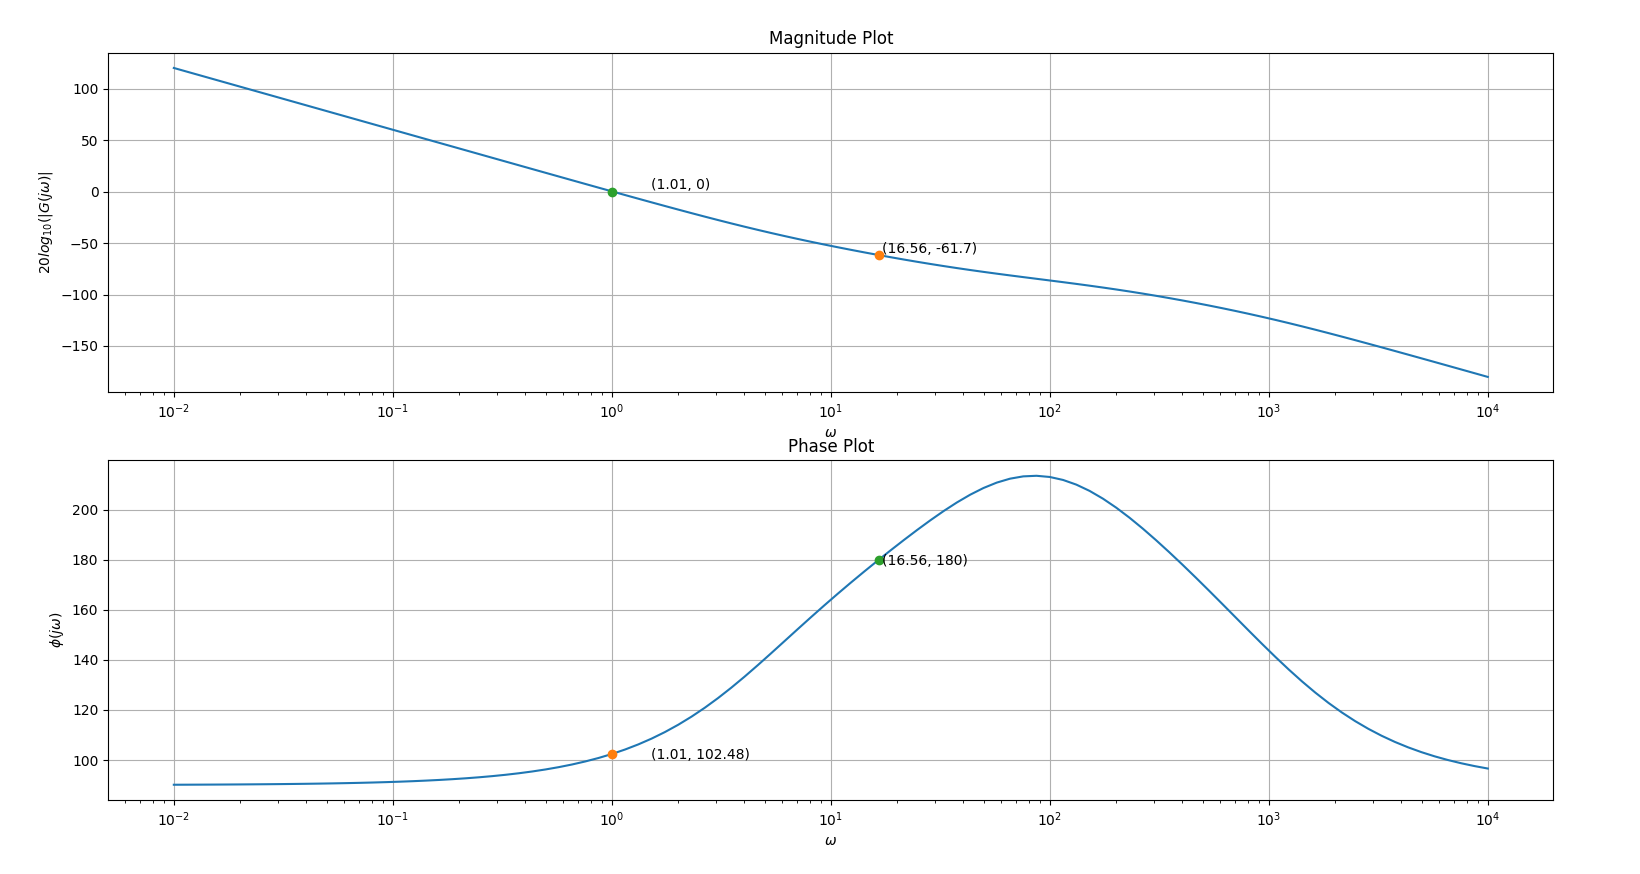
\includegraphics[width=\columnwidth]{./figs/ee18btech11039.eps}
      \caption{Bode plot}
      \label{fig:ee18btech11039}
    \end{figure}
    
    From fig. \ref{fig:ee18btech11039},
    \begin{align}
        \omega_{gc} = 16.55, \text{ Gain Margin} = -61.7 dB \\
        \omega_{pc} = 1, \text{ Phase Margin} = -77.52^0
    \end{align}
    
    The program for plotting bode plot and finding phase margin and gain margin -
    \begin{lstlisting}
        codes/ee18btech11039.py
    \end{lstlisting}
    
    \end{enumerate}
    
    
